\chapter{Referenzen und Zitate}\label{cha-ref}

Im Prinzip kann in \LaTeX auf alles referenziert werden was ein Label hat. Dies kann ein Kapitel oder Abschnitt sein, siehe Kapitel \cref{cha-ref} und Anhang \cref{app-A}, eine Formel wie die von Bernoulli \cref{eqn-bernoulli}, eine Graphik wie Abbildung \cref{fig:test_plot_1}, eine Tabelle wie  oder sogar Punkte einer Aufzählung, vgl.~\cref{enum-ebene}.

Noch eleganter sind Zitate. Man zitiert am besten auf ein Kürzel welches sich aus den ersten Buchstaben des Erstautors und der Jahreszahl zusammensetzt wie \cite{Sensoren}. Die Seitenzahl kann als Option angegeben werden \cite{Sensoren}. Verwenden Sie BibTeX, so erscheinen nur die verwendeten Literaturstellen im Literaturverzeichnis und überdies kümmert sich dann \LaTeX um die richtige Reihenfolge und Formatierung der Quellen - egal ob Buch \cite{Sensoren}, Artikel oder Dokumentation \cite{Sensoren}.

\begin{figure}[!ht]
	\centering
	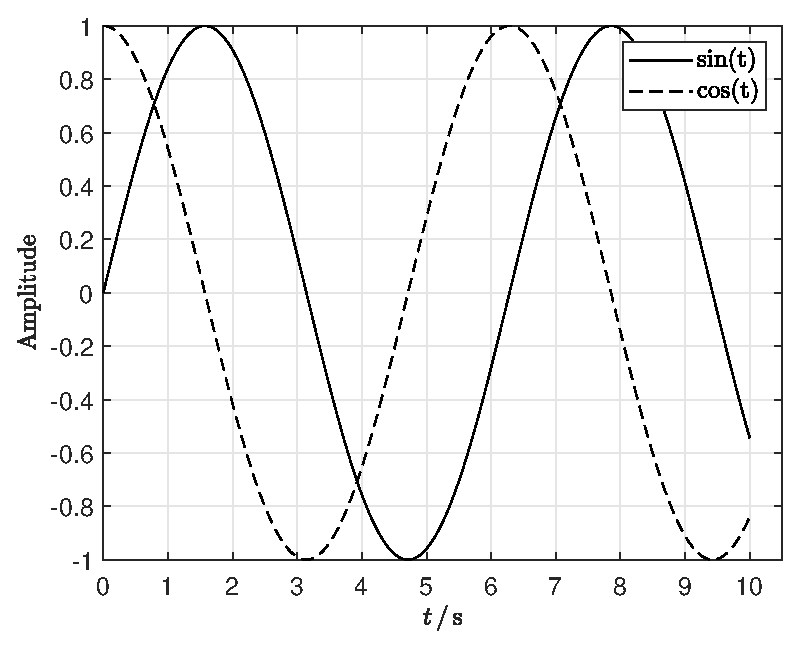
\includegraphics[width=0.6\textwidth]{img/Test_plot_1.eps}
	\caption[60\,\% der Textbreite]{Sinus- und Cosinus-Verlauf über die Zeit dargestellt.}
	\label{fig:test_plot_1}
\end{figure}

Hier ein Beispiel für Zahlen:
\begin{itemize}
	\item \num{1234,56}  % Zahl mit Dezimaltrennzeichen
	\item \SI{2}{\meter^{-1}} % Einheit m^-1 ohne Bruch
	\item \SI{1.23e4}{\newton\meter} % Exponenten mit Punkt als Produkt
	\item \SI{1000}{\kilo\ohm} % Tausender ohne Trennzeichen
\end{itemize}


Testen ob die Symbole und die Akronyms richtig funktionieren \gls{sym:C}, oder auch \gls{sym:L}.

A \gls{acr:pcb} is a fundamental component in the electronics industry and is commonly used to mechanically support and electrically connect various electronic components, including \glspl{acr:ic}. The complex impedance of an inductor is given by the formula
\begin{equation}
	Z_\mathrm{L}=\mathrm{i}\omega\gls{sym:L}
	\label{eqn:testgleichung}
\end{equation}
where $\gls{sym:L}$ is the inductance of the inductor.\par 
In \cref{fig:test_plot_1} ist ein Testplot dargestellt. und die Gleichung wird auch referenziert \cref{eqn:testgleichung}